%!TEX root = ../dissertation.tex

\chapter{Introduction}
\label{chapter:introduction}

The Internet of Things (\gls{IoT}) can be seen as a web of interconnected devices that go from everyday wearable objects into fully deployed sensor networks over a variety of architectures. Some of them provide direct connectivity of nodes to the Internet while others provide a common gateway for interfacing with external networks. In the first type of architectures, represented in Figure \ref{fig:net_overview_large}, the network nodes transmit sensing information to global access points without requiring inter-device communication. The access point can range from routers, to GSM towers or even satellites. The outgoing messages are then transmitted through the Internet to external data processing facilities, where large amounts of data from many sources are converted into useful information on demand. This information can then be accessed by the users from outside the site, also through the Internet. This type of deployments could be used, for example, in \emph{Smart Cities}, where there is the need to cover a large area with sensors.
\begin{figure}[h]
  \centering
  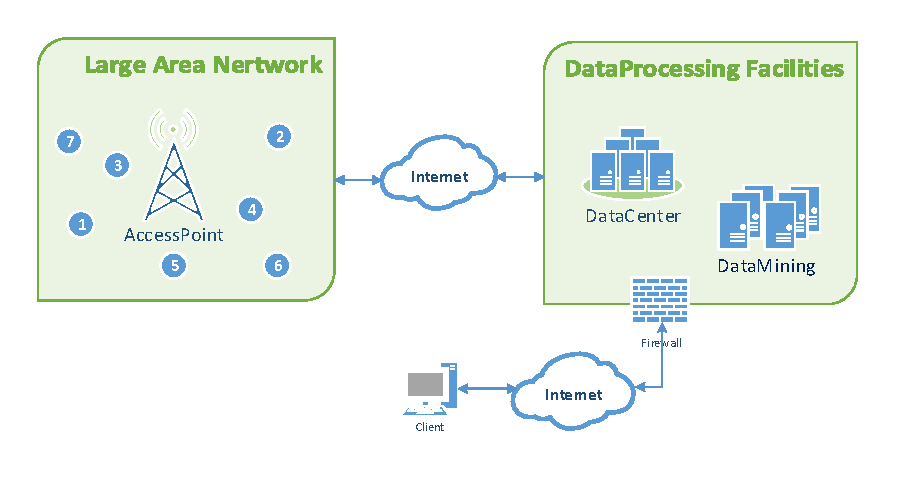
\includegraphics[width=0.85\linewidth]{figures/Network_Overview_Sparse.pdf}
  \caption{IoT Large Area Network Overview.}
  \label{fig:net_overview_large}
\end{figure}

 In the second type of architectures, illustrated in Figure \ref{fig:net_overview_small}, the sensing or actuating nodes belong to a very constrained network with specific protocols and hardware restrictions, requiring an interface device -- the \emph{border router} -- in order to communicate with external networks. After reaching the external network, incoming messages are processed to convert sensor data into useful information which is then stored or used to trigger events. This information can then be accessed by users either on the same network or by making requests through the Internet. This type of deployment could be used, for example, in a \emph{home intrusion system} where the network nodes would create a sensor network that propagates events in the case of an intrusion and the additional infrastructure would be in charge of receiving these events and notifying the police authorities.
\begin{figure}[h]
  \centering
  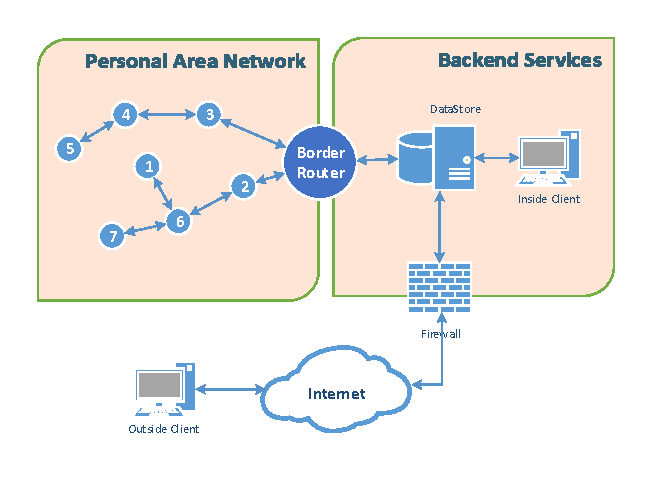
\includegraphics[width=0.8\linewidth]{figures/Network_Overview.pdf}
  \caption{IoT Personal Area Network Overview.}
  \label{fig:net_overview_small}
\end{figure}
Despite the huge variety and characteristics of these devices, one thing that they all have in common is the constrained nature that they are built upon. In order to enable the massive deployment to be expected in the near future\footnote{http://blogs.wsj.com/cio/2015/06/02/internet-of-things-market-to-reach-1-7-trillion-by-2020-idc/}, \gls{IoT} devices must be accessible and affordable, capable of operating under lossy wireless networks while being battery powered. This poses a challenge to current Internet protocols since the assumptions regarding the devices' capabilities and objectives do not hold true \cite{Trappe2015} and also raises the question: How to secure communications amongst \gls{IoT} constrained networks and devices? \\In our work we provide the answer to this question. How? Firstly, knowing that in order to allow the \gls{IoT} vision to come forward, several new network protocols have been developed across the OSI layers, each addressing and tackling the challenges involved in trying to keep the quality and assurances of more expensive protocols, on constrained systems. We do a thorough analysis of the state of the art to select the most efficient ones and group them in a power-efficient stack. Secondly, knowing that \gls{IoT} environments can range from home to enterprise or even city environments, a breach in security could potentially leak important company activity or provide information about individuals' choices and whereabouts constituting a violation of privacy \cite{Ukil2015}. To this extent, a study on existing attacks for constrained devices was conducted and available mitigation strategies investigated so that the communication model of this work could be, not only efficient, but also secure against power-draining attacks. From this investigation an additional network component was planned and implemented, providing security assurances at the cost of an increased infrastructure complexity. This managing solution -- AutoStrap -- derived its name from the necessity of a simple and automated solution. In order to accurately define the type and amount of resources needed to create such a network, we deployed our protocol stack and management station on physical hardware. After that, we performed energy, space and time profiling to provide future users with the knowledge of what kind of physical resources to deploy based on the network security characteristics.

\section{Document Overview}

In Chapter \ref{chapter:related_work} we start by analysing the state of the art regarding power-efficient protocols, battery draining attacks and mitigation strategies for constrained networks. Chapter \ref{chapter:proposed_solution} describes our solution from the objectives and architecture all the way to the implementation and execution. In order to evaluate our work, experiments were conducted on real hardware and the obtained results unveiled in Chapter \ref{chapter:evaluation}. Finally, Chapter \ref{chapter:conclusion} presents our conclusions and opportunities for future work. 

\section{Publications} 
	
This work has also been produced in the form of an article \cite{Diogo2016}, and the extended abstract of that article was accepted and presented at the INForum 2016 conference under the \emph{Internet of Things and Services} track.
